\documentclass[Second Project.tex]{subfiles}

\begin{document}

\subsection{ Μέθοδος τραπεζίου }
Η μέθοδος τραπεζίου προσεγγίζει την τιμή ενός ολοκληρώματος $\int_{a}^{b} f(x) \,dx$ μιας συνεχούς
συνάρτησης σε ένα κλειστό και φραγμένο διάστημα \textlatin{[a, b]} με χρήση εμβαδών τραπεζίων που 
προκύπτουν από την προσέγγιση της συνάρτησης $f$ από μία τεθλασµένη γραμμή. Η μέθοδος περιγράφεται παρακάτω
\begin{itemize}
    \item Έστω $\{x_{0}=a,\dots,x_{N}=b\}$, με $x_{0}<x_{1}<\dots<x_{N}$ ένας ομοιόμορφος διαμερισμός του
    \textlatin{[a, b]}, δηλαδή χωρίζουμε το \textlatin{[a, b]} σε \textit{Ν} ισομήκη υποδιαστήματα.
    \item Τότε $x_{i} = x_{0} + $κ$\frac{b-a}{N}$ ,  κ $=0,\dots,N$
    \item Υπολογίζουμε τις τιμές $f(x_{i}), i = 0,\dots,N$
    \item Σχηματίζουμε τα διαδοχικά ευθύγραµµα τμήματα µε άκρα τα $f(x_{0}),\dots,f(x_{N})$
    οπότε σχηµατίζεται µία τεθλασµένη γραµµή. 
    \item Υπολογίζουμε τα εμβαδά των Ν τραπεζίων που σχηματίζονται και μετά από πράξεις έχουμε τελικά
\end{itemize} 
\begin{equation*}
    \int_{a}^{b} f(x) \,dx \approx \frac{b-a}{2N}(f(x_{0}) + f(x_{N}) + 2\sum_{i=1}^{N-1}f(x_{i}) )
\end{equation*}
ενώ το άνω όριο του σφάλματος είναι
\begin{equation*}
    |e| \leq \frac{(b-a)^{3}}{12N^{2}}M ,
\end{equation*}
όπου
\begin{equation*}
M = max\{|f''(x)|: x\in [a, b]\}
\end{equation*}

Στο αρχείο \textlatin{\textbf{trapezoid.py}} έχουν αναπτυχθεί δύο συναρτήσεις, μία για τον υπολογισμό ενός ολοκληρώματος
από το $a$ στο $b$ για μία συνεχή συνάρτηση $f$ με την μέθοδο τραπεζίου, καθώς και μία για τον υπολογισμό του άνω ορίου του 
σφάλματος για τις προαναφερόμενες παραμέτρους. Αν καλέσουμε την συνάρτηση \textit{\textlatin{\textbf{trapezoid\_integrate}}} 
με ορίσματα την συνάρτηση του ημιτόνου, το 0, το $\frac{\pi}{2}$, το 10 και τα σημεία που αναφέρθηκαν στην εισαγωγή αυτής της
άσκησης, καθώς και την συνάρτηση \textlatin{\textbf{\textbf{trapezoid\_error\_bound}}} με τα ίδια ορίσματα εκτός της
λίστας των σημείων λαμβάνουμε τα παρακάτω
\begin{figure}[h!]
    \centering
    \captionsetup{justification=centering}
    \begin{center}
    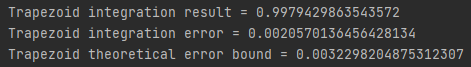
\includegraphics[scale=1]{trapezoid_results.png}    
    \caption{ Αποτελέσματα κλήσης της συνάρτησης \textit{\textlatin{\textbf{trapezoid\_integrate}}} 
    και \textit{\textlatin{\textbf{trapezoid\_error\_bound}}} στο διάστημα $[0, \frac{\pi}{2}]$.}
    \end{center}
\end{figure}

Απ' όπου παρατηρούμε ότι το σφάλμα προσέγγισης θεωρητικά είναι \\ $0.0032298204875312307$ ενώ αριθμητικά ( δηλαδή 
αφαιρώντας από την πραγματική τιμή του ολοκληρώματος, που είναι 1, και εφαρμόζοντας απόλυτη τιμή ) είναι
$0.0020570136456428134$ και τέλος, η προσεγγιστική τιμή του ολοκληρώματος με την μέθοδο τραπεζίου
είναι $0.9979429863543572$. 
\newpage
\end{document}